\documentclass[letterpaper,twoside,12pt]{report}
\usepackage[spanish]{babel}
\usepackage[utf8]{inputenc}
\usepackage{graphicx}
\usepackage{amsfonts,amsmath,amssymb,float, amsthm,mathrsfs}  
\usepackage[right=3cm,left=2cm,top=2cm,bottom=2cm,headsep= 0.7cm,footskip=0.5cm]{geometry}
\usepackage{enumerate}
\usepackage{wrapfig} 
\usepackage[rflt]{floatflt} 
\usepackage{framed}
%\usepackage[most]{tcolorbox}
\usepackage[dvipsnames]{xcolor}
\colorlet{shadecolor}{green!20}
\setlength\FrameSep{0.5ex}
\usepackage{thmtools}
\usepackage{esint}
\usepackage{cancel}
\usepackage{listings} 
\usepackage{pstricks, caption}
\usepackage[colorlinks]{hyperref}
\usepackage{csquotes}
\usepackage{fullpage}
\usepackage{enumitem}
\usepackage{etoolbox}
\usepackage{tikz}
\usepackage{tikz-3dplot}
\tdplotsetmaincoords{80}{70}
\usetikzlibrary{decorations.markings}
\usetikzlibrary{arrows,babel}
\usepackage[font=small]{caption}
\usepackage{scalerel} %\scaleto{text}{size}
\usepackage{subfigure}
\usepackage{fancyhdr}
\usepackage{comment}
\setlength{\headheight}{15pt}
\addtolength{\topmargin}{-15.49998pt}
\setlength{\headsep}{15pt}
\setlength{\footskip}{14.49998pt}
\decimalpoint
\newcommand{\grad}{^\circ}
\newlength{\drop}
\DeclareMathOperator{\sign}{sgn}
\DeclareMathOperator{\Log}{Log}
\providecommand{\norm}[1]{\left\lVert#1\right\rVert}
\newcommand{\email}[1]{\href{mailto:#1}{\texttt{#1}}}

%%%%%%%%%%%%%%Rules%%%%%%%%%%%%%%%%%%%
\newcommand{\myrule} [3] []{
    \begin{center}
        \begin{tikzpicture}
            \draw[#2-#3, ultra thick, #1] (0,0) to (0.93\linewidth,0);
        \end{tikzpicture}
    \end{center}
}
%%%%%%%%%%%%%%%%%%%%%%%%%%%%%%%%%%%%%%%

%%%%%%%%%Entornos: Teoremas, Defs,etc%%%%%%%
\theoremstyle{definition}

\newtheorem{defis}{Definiciones}[section]
\newtheorem{corolario}{Corolario}[section] 

\newtheorem{protoexample}{Ejemplo}[section]
\newenvironment{ejemplo}
   {\colorlet{shadecolor}{orange!15}\begin{shaded}\begin{protoexample}}
   {\end{protoexample}\end{shaded}}

\newtheorem*{protoproof}{Demostración}
\newenvironment{demo}
   {\colorlet{shadecolor}{blue!10}\begin{shaded}\begin{protoproof}}
   {\end{protoproof} \end{shaded}}

\newenvironment{Rdbleftbar}{%
  \def\FrameCommand{\textcolor{red}{\vrule width0.6pt}\hspace{0.15em}\textcolor{red}{\vrule width0.6pt} \hspace{0.5em}}%
  \MakeFramed {\advance\hsize-\width \FrameRestore}}%
 {\endMakeFramed}

 \newenvironment{Bdbleftbar}{%
  \def\FrameCommand{\vrule width0.6pt\hspace{0.15em}\vrule width0.6pt \hspace{0.5em}}%
  \MakeFramed {\advance\hsize-\width \FrameRestore}}%
 {\endMakeFramed}

\newenvironment{Gdbleftbar}{%
  \def\FrameCommand{\textcolor{green}{\vrule width0.6pt}\hspace{0.15em}\textcolor{green}{\vrule width0.6pt} \hspace{0.5em}}%
  \MakeFramed {\advance\hsize-\width \FrameRestore}}%
 {\endMakeFramed}
 
% With parskip

\usepackage[indent=0.6cm]{parskip}

\declaretheorem[%
name            =Teorema,%
numberwithin=section,
postheadhook    =\vspace*{\parskip} \begin{Rdbleftbar}\vspace*{-5pt},%
prefoothook     =\vspace*{-1pt}\end{Rdbleftbar}%
]{teorema}

\declaretheorem[%
name            =Definición,%
numberwithin=section,
postheadhook    =\vspace*{\parskip}\begin{Bdbleftbar}\vspace*{-5pt},%
prefoothook     =\vspace*{-1pt}\end{Bdbleftbar}%
]{defi}

\declaretheorem[%
name            = Proposición,%
numberwithin=section,
postheadhook    =\vspace*{\parskip}\begin{Gdbleftbar}\vspace*{-5pt},%
prefoothook     =\vspace*{-1pt}\end{Gdbleftbar}%
]{propo}  

\declaretheorem[%
name            = Lema,%
numberwithin=section,
postheadhook    =\vspace*{\parskip}\begin{Gdbleftbar}\vspace*{-5pt},%
prefoothook     =\vspace*{-1pt}\end{Gdbleftbar}%
]{lema}   
%%%%%%%%%%%%%%%%%%%%%%%%%%%%%%%%%%%%%%%%%%%%%%

%%%%%%%%%%%%Fancy Chapters%%%%%%%%%%%%%%%%%
%Options: Sonny, Lenny, Glenn, Conny, Rejne, Bjarne, Bjornstrup
\usepackage[Lenny]{fncychap}
%%%%%%%%%%%%%%%%%%%%%%%%%%%%%%%%%%%%%%%%%%%

\fancypagestyle{mystyle}{

\fancyhf{}
\fancyhead[LE]{\nouppercase{\rightmark}}
\fancyhead[RO]{\nouppercase{\leftmark}}
\fancyfoot[LE,RO]{\hfill\thepage\hfill}
}

\spanishdecimal{.}

\begin{document}

\sffamily
\begin{titlepage}
 \drop=0.1\textheight
    \centering
    \vspace*{\baselineskip}
    \rule{\textwidth}{1.6pt}\vspace*{-\baselineskip}\vspace*{2pt}
    \rule{\textwidth}{0.4pt}\\[\baselineskip]
    {\rmfamily\scshape\Huge Computación Científica II}\\[0.2\baselineskip]
    \rule{\textwidth}{0.4pt}\vspace*{-\baselineskip}\vspace{3.2pt}
    \rule{\textwidth}{1.6pt}\\[\baselineskip]
    {\Large Autor: \par}
{\Large Martín Aedo \par}
\vfill
{\large Agosto 2026 \par}
{\large v2.0 \par}
\end{titlepage}

\chapter*{Prefacio}


\emph{Este documento es un apunte redactado por Martín Aedo, su uso es destinado para fines académicos y de estudio para el curso de Computación Científica II o de algun otro caracter, dictado por el Prof. G. Rubilar del departamento de Física de la Universidad de Concepción.}

\emph{En caso de comentarios, correcciones o sugerencias, se puede contactar a través del correo electrónico: \email{maraedo2022@udec.cl}}
\tableofcontents

\pagestyle{mystyle}

\chapter{Ecuaciones Diferenciales Ordinarias}

\section{Ecuación diferencial Masa Resorte}

En el mundo de la física se resuelve problemas relacionados a describir movimientos, como por ejemplo los oscilatorios. Un sistema clásico de este es el de una masa atada a un resorte, modelar y predecir este sistema es un trabajo largo si solo nos enfocaramos en ver instantes de este a lo largo del tiempo, en cambio si vieramos este sistema como uno repetitivo o uno cíclico se reduciria ampliamente el procedimiento.

Partamos primero por las fuerzas que se aplican en el sistema:

\begin{itemize}
    \item Fuerza de gravedad $F_{g}= mg$
    \item Fuerza restauradora del resorte $F_{k}=-kx$
\end{itemize}

Las cuales al insertarlas en un sistema de cuerpo libre, tal que colgamos el cuerpo al resorte, resultarian en direcciones opuestas, por lo cual, si quisieramos describir finalmente le movimiento de un resorte (Fuera del estado de equilibrio), su ecuación resultante sería:

\begin{align}
    ma = ky - mg  \nonumber\\
    m \frac{d^2 y}{dt^2} = - ky - mg \nonumber \\
    m \frac{d^2 y}{dt^2} + ky = -mg  \nonumber \\
    \frac{d^2 y}{dt^2} + \frac{k}{m} y = -g \nonumber
\end{align}

Usaremos la definición de frecuencia angular de tal forma que $\omega^2 = \frac{k}{m}$ resultando la ecuación final como:

\begin{equation}
    \frac{d^2 y}{dt^2} + \omega^2 y =-g \nonumber
\end{equation}

Resolviendo esta EDO nos resulta la posición y velocidad igual a :

\begin{align}
    y(t) = (y_{0} +\frac{g}{\omega^2})cos(\omega t) + \frac{v_{0}}{\omega}sin(\omega t) -\frac{g}{\omega^2}  \nonumber \\
    v(t)= -(y_{0} +\frac{g}{\omega^2}) \omega sin(\omega t) + v_{0} cos(\omega t) \nonumber
\end{align}
Si se utiliza las soluciones numéricas de ecuaciones diferenciales ordinarias, usando la frecuencia angular igual a $1 [\frac{rad}{s}]$ y la aceleración de gravedad es de $9,81 [\frac{m}{s^2}]$ resultan en:

\noindent
\begin{minipage}[t]{0.48\textwidth}
    \centering
    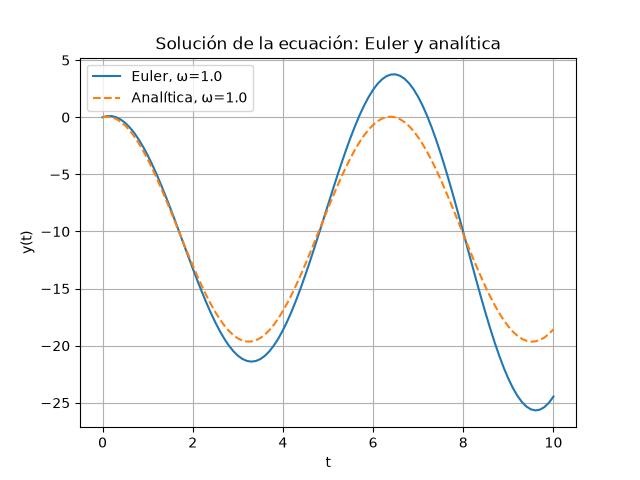
\includegraphics[width=\linewidth,height=0.19\textheight,keepaspectratio]{Figures/Euler_1.png}
    \captionsetup{hypcap=false}
    \captionof{figure}{Método de Euler comparado con la solución analítica.}
    \label{fig:euler}
\end{minipage}
\hfill
\begin{minipage}[t]{0.48\textwidth}
    \centering
    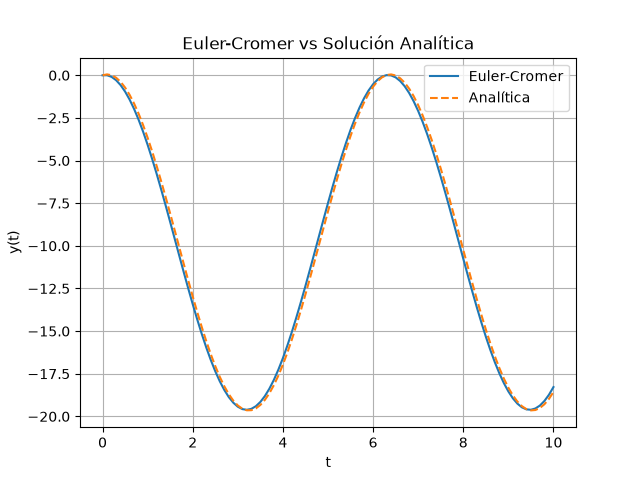
\includegraphics[width=\linewidth,height=0.19\textheight,keepaspectratio]{Figures/Euler_cromer_1.png}
    \captionsetup{hypcap=false}
    \captionof{figure}{Método de Euler-Cromer comparado con la solución analítica.}
    \label{fig:euler-cromer}
\end{minipage}

\par\vspace{0.5em}
\noindent
\begin{minipage}[t]{0.48\textwidth}
    \centering
    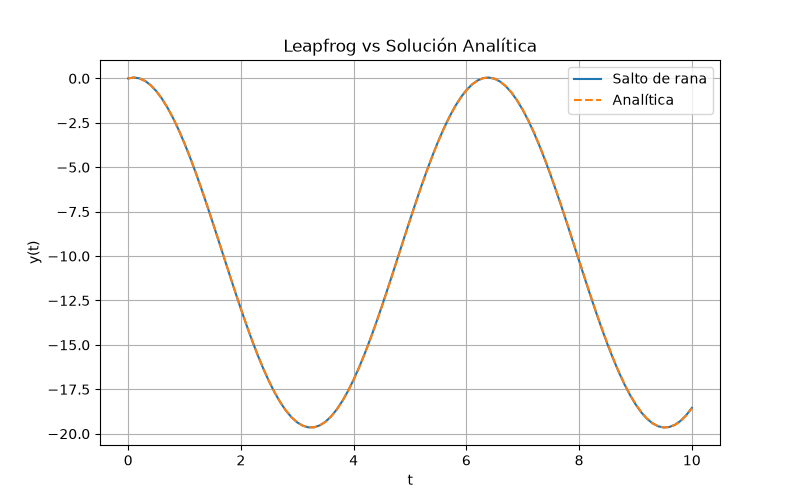
\includegraphics[width=\linewidth,height=0.19\textheight,keepaspectratio]{Figures/Leapfrog_1.png}
    \captionsetup{hypcap=false}
    \captionof{figure}{Método de salto de rana comparado con la solución analítica.}
    \label{fig:salto-rana}
\end{minipage}
\hfill
\begin{minipage}[t]{0.48\textwidth}
    \centering
    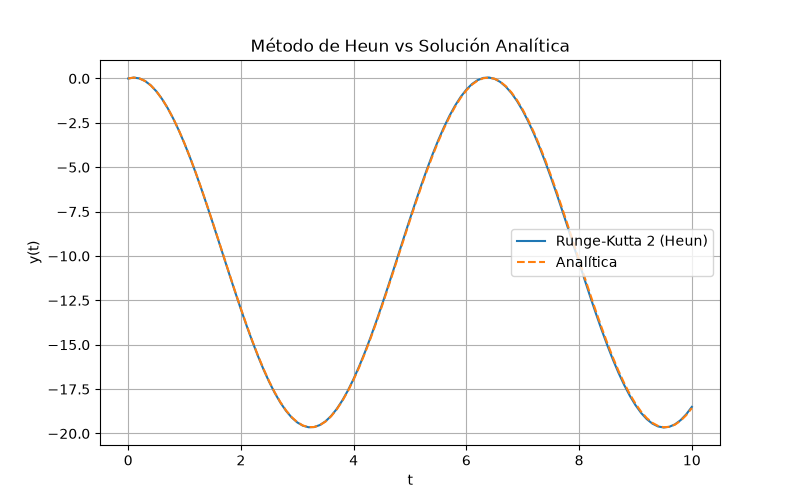
\includegraphics[width=\linewidth,height=0.19\textheight,keepaspectratio]{Figures/Heun_1.png}
    \captionsetup{hypcap=false}
    \captionof{figure}{Método de Heun (Runge-Kutta de segundo orden) comparado con la solución analítica.}
    \label{fig:heun}
\end{minipage}

\par\vspace{0.5em}
\noindent\hfill
\begin{minipage}[t]{0.48\textwidth}
    \centering
    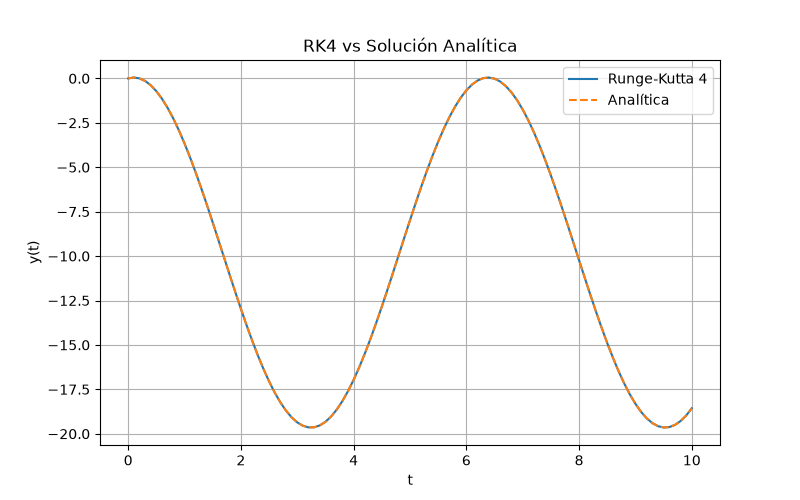
\includegraphics[width=\linewidth,height=0.19\textheight,keepaspectratio]{Figures/RK4_1.png}
    \captionsetup{hypcap=false}
    \captionof{figure}{Método de Runge-Kutta de cuarto orden comparado con la solución analítica.}
    \label{fig:rk4}
\end{minipage}
\hfill\null


Concluyendo que el método más aproximado a la solución analítica es el Método de Runge-Kutta de 4to orden.

Con respecto a la energía del sistema podemos definirla como:

\begin{equation}
    E_{t} = E_{c} + E_{k} + E_{g} \nonumber
\end{equation}

Siendo cada componente:

\begin{itemize}
    \item $E_{t}$: Energía del sistema
    \item $E_{c} = \frac{1}{2} m v^2 $: Energía cinética
    \item $E_{k} = \frac{1}{2} k y^2 $: Energía potencial elástica
    \item $E_{g} = m g y $: Energía potencial gravitatoria
\end{itemize}

Tal que al evaluar cada una de las soluciones numéricas en la energía nos resulta la \hyperref[fig:energia]{siguiente gráfica}:

\begin{figure}[H]
    \centering
    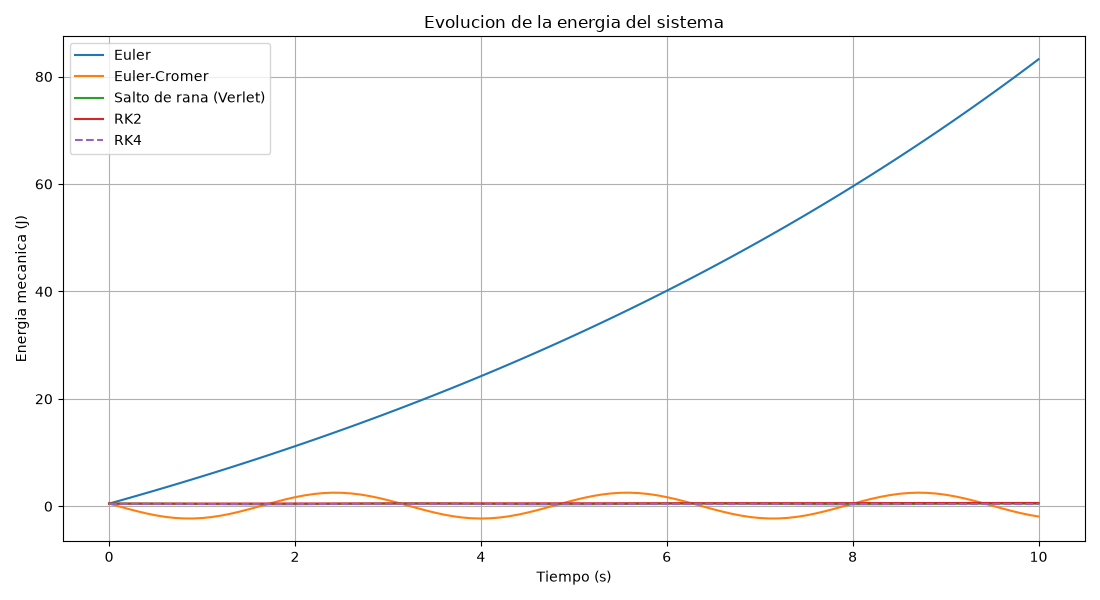
\includegraphics[width=0.8\textwidth]{Figures/Energía_1.png}
    \captionsetup{hypcap=false}
    \caption{Energía total del sistema calculada con los distintos métodos numéricos.}
    \label{fig:energia}
\end{figure}

En un sistema masa-resorte ideal, sin fuerzas disipativas, la energía mecánica total debe conservarse: la energía cinética y las energías potenciales elástica y gravitatoria se transforman entre sí, pero su suma permanece constante. En la gráfica, los métodos de salto de rana, Heun y Runge-Kutta de cuarto orden mantienen la energía cerca de su valor inicial durante el intervalo considerado. Euler-Cromer presenta oscilaciones acotadas, mientras que Euler muestra un aumento sostenido de la energía, lo que evidencia una acumulación importante de error numérico. Por lo tanto, para esta simulación, Runge-Kutta de cuarto orden ofrece un comportamiento energético consistente con la conservación esperada y Euler es el método que más se desvía.

\subsection*{Conclusión general}

El análisis del sistema masa-resorte muestra que las ecuaciones diferenciales ordinarias permiten describir su movimiento y comparar soluciones numéricas con la solución analítica. Los resultados dependen del método utilizado: en las condiciones simuladas, Runge-Kutta de cuarto orden es el que mejor se aproxima a la solución analítica y conserva más adecuadamente la energía, mientras que Euler acumula errores apreciables con el tiempo. En consecuencia, la elección del método numérico es importante para obtener resultados fiables; también conviene considerar el tamaño del paso temporal y verificar que las magnitudes físicas relevantes, como la energía, mantengan el comportamiento esperado.


\nocite{*} % Referencia todo, incluso lo que no está citado.
\bibliographystyle{plain}
\bibliography{Referencias}

\end{document}